\chapter{Kernel CN:\ Grammar}%
\label{chap:kernel-grammar}

\margintoc%

\kl{CN} and \kl{Kernel} CN have different grammars. This is because \kl{CN} is
intended to be used by C programmers, whereas \kl{Kernel} CN is for type
theorists, thus more convenient to understand and work with as a formalism. The
primary differences are (a) \kl{CN} is implemented over (a version of)
\kl{Core}, whereas the \kl{kernel} is defined over a let-normalised
\kl{ResCore} (b) \kl{CN}'s grammar of types is close to the surface syntax and
so each construct serves many purposes whereas the \kl{kernel}'s grammar of types
is more traditional and each construct only serves one purpose.

In this chapter I will present the relevant parts of \kl{CN}'s syntax of
predicate definitions and assertions, and the \kl{kernel}'s syntax of types and
relevant terms, with a particular focus on explicit resource terms.

\section{Kernel CN types}

\begin{figure}
    \small
    \grammartabularSTY{
        \cnfon{}\cninterrule{}
        \cnret{}\cnafterlastrule{}
    }
    \caption{\kl{Kernel CN} function and return types.}\label{fig:kernel-fun-ret}
\end{figure}

\cref{fig:kernel-fun-ret} show the grammar of function types $\cnnt{fun}$ which
include both pre- and postconditions, and return types ${ret}$, which
represents postconditions. Where the \kl{CN} grammar pre- and postconditions
are a flats list of ${conditions}$, these types are nested and have quantifiers
to make explicit their scoping, specifically that the variables bound in the
precondition are available for use in the postcondition. This is necessary
because these types depend on computational values, and so, for example, a call
to a function needs to propagate the symbolic or concrete function arguments
into the rest of a pre- and postcondition (via a spine judgement).

In order, both include: quantification over computational (program) values,
quantification over logical (ghost) values, separating implication/conjunction
for assertions about the heap,\sidenote{TODO\@: Should I change this (back) to
$\otimes$ and $\multimap$? Or would that be confusing? I also don't
have `multimap' in my maths font.} and logical implication/conjunction for pure
assertions (in a linear context, about an empty heap).

Though this seems like a large departure from the syntax given in
\cref{fig:cn-grammar}, the mapping into this is straightforward, and helps
clarify what each \kl{CN} surface construct represents in more familiar,
type theoretic terms.

Before I explain this mapping, there is one more key component left to explain:
\emph{resource types}. As seen in~\cref{fig:kernel-res}, they are type for
separation logic assertions, which will be treated linearly. The constructs are
quite standard, except for the only mention of branching in any of the types,
with the \emph{ordered} disjunction, to prevent the need for backtracking,
rather than the usual $\vee{}$.

For ease of implementation and formalisation, we do not have branching for pre-
and postconditions and function/return types, but this does not affect
expressiveness because these can be embedded into the resource types. Note that
in the formalisation, the branching is not restricted to the top-level in
predicate definitions, but can occur directly in function types, and can be
arbitrarily nested. This makes defining predicates to represent tagged unions
more succinct, and allows for opening predicates in more cases.

Predicates ${pred}$ and iterated predicates ${qpred}$ are simple ${pred\_term}$
and ${qpred\_term}$ with output arguments, as seen in~\cref{fig:kernel-qpred}.
I will explain why I factored out ${pred\_term}$ and ${qpred\_term}$ in
\nameref{sec:res-terms}. For now, I will draw attention to the fact that
where there is a distinction between \cninline{Owned} and \cninline{Block} in
the surface syntax, the formalisation tracks whether or not a points-to has
been initialised in a symbolic \emph{record} field ${.init}$, whose type
mirrors the structure of the C type, i.e.\ with leaves which are booleans, and
branches which are records or arrays. This allows for more fine-grained control
over reading and writing \emph{partially} (and completely) uninitialised reads
of structs/unions,\sidenote{\url{https://www.cl.cam.ac.uk/~pes20/cerberus/notes98-2018-04-21-uninit-v4.html\#reads-of-partially-uninitialised-structsunions-as-a-whole}% chktex 8
\\ Though honestly I could just get rid of this because it would be simpler.}\label{sn:partial-init-read}
as allowed by the C standard.

\begin{figure*}
    \small
    \raggedright{}
    \grammartabularSTY{%
        \cnpredXXname{}\cninterrule{}
        \cnpredXXterm{}\cninterrule{}
        \cnqpredXXterm{}\cnafterlastrule{}
    }
    \begingroup%
    \renewcommand{\cnprodline}{\cnprodlineCommentNewline}
    \grammartabularSTY{%
        \cnqpred{}\cnafterlastrule{}
    }
    \endgroup%
    \caption{\kl{Kernel CN} predicate and iterated predicate terms (without
        output arguments) and types (with output arguments). The formalisation
        is set up with some syntactic sugar (marked with $\mathsf{S}$) to make
        the meanings of these constructs more intuitive.}\label{fig:kernel-qpred}

\end{figure*}

\begin{figure*}
    \small
    \grammartabularSTY{%
        \cnres{}
    }
    \caption{\kl{Kernel CN} resource types, a linear type for separation logic
        assertions.}\label{fig:kernel-res}
\end{figure*}

\section{Desugaring \kl{CN} types into \kl{kernel} types}\label{sec:desugaring}

All judgements in the formalisation which have a natural bidirectional
interpretation have the information they are synthesising highlighted with
\colorbox{pink!30}{light pink} background. The grammars presented below will
refer to ${term}$, ${iguard}$, ${ptr}$, ${init}$, ${value}$, ${iarg}$, ${oarg}$
(and later, ${alloc}$). These are all simply aliases for pure (SMT) terms, used
so that the roles of these terms in different productions, especially ones
productions which refer to multiple instances of them, are clearer. \intro{Base
types}, represented by $\beta$ or ${bty}$ are simply the types of such terms.

Desugaring \kl{CN} types into \kl{Kernel CN} starts with the C functions, which
map their parameters into computational variables in function types, or with
predicate definitions, which map their parameters into essentially a
$\lambda$-abstraction over a resource type (\cref{fig:prepost-to-kernel}). To
be clear, this is merely quantifying over pure (SMT) terms in the type, rather
than any higher-order assertions about the shape of the heap.

\begin{figure*}[tp]
    \small
    \raggedright{}
    \cndefnSpecXXUserDef{}
    \cndefnSpecXXPredDef{}
    \caption{\kl{CN} to \kl{Kernel CN} pre- and postcondition and predicate
        definition desugaring. For the C functions, each C argument is bound to
        a computational argument, with a base type $\beta_\tau$ corresponding
        to the C type $\tau$. Predicate definitions simply abstract pure (SMT)
        terms over resources.}\label{fig:prepost-to-kernel}
\end{figure*}

Desugaring preconditions into function types requires the postcondition to be
desugared first; because that is similar to precondition desugaring, I will
omit it for space. Abbreviations are simply substituted into the function
type.\sidenote{In the implementation, for better error messages, they are bound
to a fresh variable and constrained with an equality constraint.}\label{sn:abbrev}
Constraints are mapped into logical implications. The formalisation can handle
ifs directly in the precondition, unlike the surface syntax which allows ifs to be placed
only at the top-level of a predicate (\cref{sec:restriction-branching}).

The monadic binding \cninline{take id = ..} is always translated into a logical % chktex 26
quantification over the output argument of the (iterated) predicates. Because
all the predicate definitions are guaranteed to be precise, all the logical
quantifications can be inferred when required.

\begin{figure*}[tp]
    \small
    \raggedright{}
    \cndefnSpecXXNormArg{}
    \caption{\kl{CN} to \kl{Kernel CN} precondition desugaring. I use $x \equiv e$
        to introduce $x$ as an abbreviation for $e$ when $e$ is a long term.
        Postcondition desugaring is similar, and thus omitted.}\label{fig:precond-to-kernel}
\end{figure*}

Desugaring predicate definitions is similar. Because the grammar is used in two
contexts, inside a pre- or postcondition where a return is not allowed, and in
a predicate definition where a return is allowed, the desugaring is
parameterised over whether or not a return is expected. If one is not, then the
resource is simply an $\mathsf{emp}$, otherwise it is an equality constraint,
as shown in \cref{fig:monad-sl}. Outputs of (iterated) predicates are always
assumed to be of the shape of a record for uniformity, which I will justify
later. Abbreviations are also substituted in.\sidenote{As in note~\ref{sn:abbrev}.}
Because pure (SMT) terms are syntactically stratified out of
the impure ones, they are embeded directly into a resource type (separation
logic assertion) with $\astRef{}$. Ifs in the syntax are translated into ifs in
the resource type grammar, with some adjustment based on whether it occurs in a
terminal place; no returns are expected/allowed in non-terminal
ifs. This restriction side steps the need for a more complicated
destination-passing style~\sidecite{shaikhha2017destination} transformation to
translate the semantics of early-returns into precise separation logic
assertions. Lastly, as before, the monadic binding \cninline{take id = ..} is % chktex 26
always translated into a logical quantification over the output argument of the
(iterated) predicate.

\begin{figure*}[tp]
    \small
    \raggedright{}
    \cndefnSpecXXRes{}
    \caption{\kl{CN} to \kl{Kernel CN} user-defined predicate desugaring.}\label{fig:pred-to-kernel}
\end{figure*}

\section{ResCore}\label{sec:rescore}

Not only is the formalisation defined over a desugared representation of types
from the surface \kl{CN} syntax, it is also defined over the let-normal form of
the \kl{Core} grammar
(\cref{fig:pure-core-grammar,fig:effectful-core-grammar}). By let-normal, I
mean an A-normal~\sidecite{flanagan1993essence} form which is closed under
substitution.

Specifically, it syntactically stratifies values and
expressions from which we would like to \emph{synthesise} type information, and
top-level values and expressions against which we would like to \emph{check} a
given type. This applies to both pure and effectful fragments, leading to a
four-fold distinction in the let-normal form of the grammar.

This dramatically simplifies presenting and working with the type system, because:
\begin{itemize}
    \item \coreinline{undef()}. In typing this, it is necessary to give is a % chktex 36
        checking rule, since control flow is required to not reach that point
        (\cref{fig:core-ub-typing}).
    \item \textbf{Control flow}. Here too, we would also very much like to use
        a checking rule, since this would sidestep the need to synthesise
        least-upper bound types for join-points after all \kl{Core}
        \coreinline{if}-expressions (or require annotations on them), at the
        cost of accepting a combinatorial explosion in typing all subsequent
        expressions.
    \item \textbf{Lets}. In typing these, we would also very much like to use a
        \emph{synthesis} rule for the bound expression, since that removes the
        need for an annotation to be placed on the binder there.
    \item \textbf{Memory actions}. These too are well-suited to synthesis, since
        they can manipulate they manipulate the resource context via the
        resources types they will synthesise.
\end{itemize}

Initial implementations of \kl{CN} did a full A-normalisation of Core, but this resulted
in far too many logical variables being created (one for each intermediate
sub-expression) and these were very difficult to relate back to the source
program in concrete counter-examples produced by the SMT
solver.\sidenote{Location information was not tracked properly either so this
was doomed.} Hence, this was
removed.\sidenote{\href{https://github.com/rems-project/cerberus/commit/21808139bda2ee320756c71eb22dbd57d0986f97}{Commit
21808139.}}\label{sn:rm-anorm}

The way that \kl{CN} currently manages the flow of information is by explicitly
passing around continuations; when it comes across any expression which is
treated as a top-level one in \kl{let-normal Core}, it simply does the appropriate
checks and then \emph{drops} the continuation.\sidenote{\href{https://github.com/rems-project/cerberus/commit/350fefc675626dcc69c7adc9edea30ff9687b752}{Commit 350fefc6.}}\label{sn:use-conts}
This makes the code more fragile but saves the need for maintaining another large
syntax tree which needs pretty-printers, debug printers, source location
mappings and so on.

Since it would require more complex fractional permissions, I left out
let-normalising the constructs related to C's loose evaluation order.\sidenote{%
\coreinline{neg()}, \coreinline{unseq()}, \coreinline{let weak}, % chktex 36
\coreinline{let strong}, \coreinline{bound()}, \coreinline{nd()}, % chktex 36
\coreinline{par()}.} However, this also means the formalisation glosses % chktex 36
over the fact that those constructs can contain each other in a semantically
meaningful way, such that flattening out that nesting seems impossible. A
solution would be to require type annotations on any situation which requires
top-level expressions to be nested inside one another.

Indeed, as I shall show in \nameref{chap:kernel-soundness}, annotations on
nested top-level expressions are required, though only for proving type
preservation for function calls to pure Core functions, effectful Core
procedures, and elaborated C functions. And as I will demonstrate in
\nameref{chap:kernel-alternative}, it seems very difficult to avoid some sort
of normalisation (and associated control flow explosion) somewhere in the type
system in the presence of join-points and early returns in sub-expressions.

For now, I will confine my discussion of the let-normal grammar to top-level
expressions (full details for both nested and top-level expressions are
available in the appendix). Pure expressions include things such as pure values,
datatype values, pointer arithmetic for arrays (in \kl{de facto}, not \kl{ISO})
and struct/union members, boolean negation, binary operations and relations, function
calls and assertions. Top-level values and expressions are in
\cref{fig:kernel-tp}. As mentioned earlier, constructs where control flow
should not reach, such as \coreinline{undef()} must be in a checking % chktex 36
judgement, so top-level values consists of them and regular pure values lifted
to the top.

\begin{figure*}
    \small
    \grammartabularSTY{%
        \cntpval{}\cninterrule{}
        \cntpexpr{}\cnafterlastrule{}
    }
    \caption{Top-level pure values and expressions in ResCore.}\label{fig:kernel-tp}
\end{figure*}

Top-level effectful values are the same as top-level pure values.
Effectful values and expressions are further split into \intro{sequenced}
expressions and \intro{indeterminately} sequenced expressions. Sequenced
expression include only C function calls and Core procedure calls.
As shown in \cref{fig:kernel-is-expr}, \kl{indeterminately} sequenced
expressions include annotated top-level values, memory operations, and explicit
terms to pack or unpack predicates (I will explain explicit resource terms in
\cref{sec:res-terms}).

\begin{figure}[h]
    \small
    \grammartabularSTY{%
        \cnisXXexpr{}\cnafterlastrule{}
    }
    \caption{Indeterminately sequenced expressions in ResCore.}\label{fig:kernel-is-expr}
\end{figure}

Sequenced top-level effectful expressions (\cref{fig:kernel-texpr}) are
simply the constructs which mention a pure expression inside them; you can see
that the bound expression in a \coreinline{let}, the scrutinee of a
\coreinline{case}, the condition of an \coreinline{if}, as well as the
arguments to \coreinline{run} are contain pure expressions
(\cref{fig:effectful-core-grammar}).

However, these are mutually defined with \kl{indeterminately} sequenced
top-level expressions (\coreinline{let weak} and \coreinline{let strong}), for
which as I mentioned before, I do not have accurate support. The mutual
recursion is achieved via the $\mathit{texpr}$ production.

\begin{figure*}[tp]
    \small
    \grammartabularSTY{%
        \cnseqXXtexpr{}\cninterrule{}
        \cntexpr{}\cnafterlastrule{}
    }
    \caption{Top-level expressions in ResCore.}\label{fig:kernel-texpr}
\end{figure*}

\section{Resource terms}\label{sec:res-terms}

One of the key initial motivations for formalising (and ultimately
implementing) a smaller kernel for \kl{CN} was to have a stronger safety net
underneath its resource inference algorithm, both at the time and for all
future inference algorithms. The hope was that this would allow us to iterate
quickly and boldly on the algorithms, with much less worry about introducing
unsoundness.

This did not materialise because \kl{CN} moved away from A-normalising
\kl{Core}, adopted a continuation-passing style, and changed its approach to
resource inference.\sidenote{See notes~\ref{sn:rm-anorm},~\ref{sn:use-conts}
and~\ref{sn:new-inf}} Another large hurdle was that it would have required
significant engineering effort to refactor the internal \intro[AST]{abstract
syntax trees} (ASTs).

Yet, the effort was still fruitful since it brought extra clarity to questions
around the implementation (\nameref{chap:inform-impl}) and inspired ideas on
how to feasibly and gradually transition the most subtle and complex parts of
\kl{CN} (either now, or in the future) to a
proof-assistant (\nameref{sec:better-foundations}).

The key concept which makes this possible is to include explicit (linearly
typed) terms for both resources \emph{and operations on them} in the grammar of
\kl{ResCore}. Though this is not a new
concept~\sidecite{xi1999dependent,cui2005ats,ahmed2007l3}, its application in a
separation logic settings appears to be so, because these sorts of
manipulations are usually done manually in an interactive proof-assistant and
recorded as tactics in a proof script \emph{external} to the program being
verified. In {kernel CN}, these \intro{resource terms} serve many purposes:
\begin{itemize}
    \item \textbf{Resource annotation.} They act as resource type annotations
        on constructs which require them.
    \item \textbf{Primitives.} They clarify the smallest units of
        resources and operations on them.
    \item \textbf{Bookkeeping.} They act as a log of the sequence of operations
        required to (soundly) manipulate the resource context from one symbolic
        state to another.
\end{itemize}

Of course, as with logical (ghost) terms, resource terms must be added with
care to the language to ensure erasure; they must not affect the control flow,
the values computed, or the memory events executed. This is easy to see by the
fact that resource terms are only placed on the memory actions for reading,
writing or destroying a heap location, and for memory operations involving
pointers which require checks that pointers are live (\cref{fig:res-term-constructs}).

\begin{marginfigure}
    \centering
    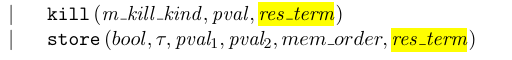
\includegraphics{figures/kernel-res-term-1}
    
\includegraphics{figures/kernel-res-term-2}
    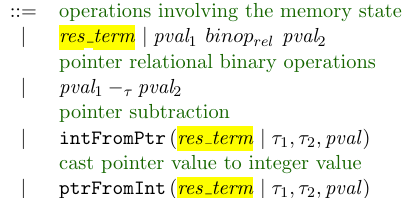
\includegraphics{figures/kernel-res-term-3}
    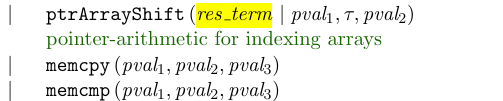
\includegraphics{figures/kernel-res-term-4}
    \caption{Constructs in \kl{ResCore} extended to accommodate
    explicit resource terms.}\label{fig:res-term-constructs}
\end{marginfigure}

To be clear, \kl{CN} \emph{users} are still not required to explicitly provide
any resource terms; they are used so that any algorithms for \emph{inferring}
them can be rephrased naturally as algorithms for \emph{elaborating} a program
\emph{without} resource annotations into one \emph{with} them.

Another advantage of having explicit resource terms in the grammar of
\kl{ResCore} is that this lets the heaps in the dynamic semantics be
represented more abstractly, whilst still precisely controlling their
transformations according to the reduction rules of the resource terms. This
additional modularity, whilst a bit confusing at this stage, will be seen to
pay off later when discussing the proof of soundness for the CN-VIP memory
object model (\cref{sec:cn-vip-soundness}).

\cref{fig:res-terms} shows the resource terms of \kl{ResCore}. There are
\emph{several} side conditions for each of the operations the terms represent,
which I will show in \nameref{sec:typing-res-terms}, but for now it suffices to
explain just the intuition. Terms $\mathsf{emp}$ and
$\mathsf{term}$ are introduction forms for the types $\mathsf{emp}$ and pure
assertions $\mathit{term}$, and they have corresponding forms for eliminating
them too. Variables are also resource terms and patterns, for any resource
type. Terms $\mathit{pred\_term}$ and $\mathit{qpred\_term}$ introduce
$\mathit{pred}$ and $\mathit{qpred}$ types respectively (the only difference
between the two is that the latter also carry their output arguments). Angle
brackets $\langle \_ , \_ \rangle$ and $\mathsf{pack}$ are introduction forms
for the separating conjunction $\astRef{}$ and $\exists$ types respectively,
and they have corresponding eliminators too.

Ordered-disjunctions can be introduced by \emph{any} resource term, and
eliminated by any resource pattern.

The following terms are all operations on predicates. Types for
user-defined predicates are introduced and eliminated by the $\mathsf{fold}$
construct, so that definitions of predicates can be hidden or exposed as required
(necessary because we need and allow predicates to be recursive). The
$\mathsf{implode}$ and $\mathsf{explode}$ constructs are for transforming from
and to an $\mathsf{Owned}\langle \mathtt{struct} \mathit{tag} \rangle$ predicate
(which, in kernel CN, represents both \cninline{Owned<ct>} and
\cninline{Block<ct>} from the surface syntax); the first consumes ownership of
a struct and produces ownership of its members, the second does the inverse.
Analagously for $\mathsf{iterate}$ and $\mathsf{congeal}$, the former consumes
ownership of a fixed-size array, and produces ownership to each of its members,
whereas the latter does the inverse.

The remaining terms are all operations on iterated predicates. The
$\mathsf{break}$ operation indexes an iterated predicate to move ownership out
of it, whereas the $\mathsf{glue}$ operation does the inverse. The
$\mathsf{inj}$ operation introduces a singleton (non-empty) iterated
predicate.\sidenote{I chose a singleton introduction form rather than an empty
    one to enforce the invariant that all iterated predicates in the typing
    context are guaranteed to be non-empty. I do not believe this makes a
    material difference to soundness, but it reduces redundant lookups in the
    resource context, and avoids the need of inventing default values for empty
    arrays in the SMT problem. However, due to the mismatch between finite
    arrays in C, and total maps in SMT theories, the difference does seem to
    affect usability in the implementation
(\href{https://github.com/rems-project/cerberus/issues/729}{issue \#729}).
TODO\@: allow empty arrays and require the array value to be put in the rather
term than assume default.}
Lastly, the $\mathsf{chop}$ operation splits an iterated predicate along a
given index guard $\mathit{iguard}$. As mentioned in
\nameref{sec:monadic-syntax}, to preserve decidability by not inferring
quantified constraints, the type system does not support merging arrays.

\begin{figure*}[tbp]
    \centering
    \small
    \grammartabularSTY{%
        \cnresXXterm{}\cninterrule{}
        \cnpredXXops{}\cninterrule{}
        \cnresXXpat{}\cnafterlastrule{}
    }
    \caption{Explicit resource terms in \kl{ResCore}.}\label{fig:res-terms}
\end{figure*}

